\section{Justificación de las Pruebas}

Todas las encuestas incluidas en esta sección, junto con sus respectivos gráficos se encuentran a disposición en \hyperref[Anexos]{Anexos}.

\subsection{Encuesta: Impacto del Dominio del Inglés en la Vida Académica y Profesional}

Este formulario se diseñó con el propósito de analizar el impacto que tiene el dominio (o su ausencia) del inglés en la vida académica y profesional de las personas. Se busca validar la idea de que la competencia idiomática influye significativamente en el acceso a nuevas oportunidades tanto académicas, profesionales y sociales.

\subsection{Encuesta: Prueba de usabilidad English with Ogloc}

Se diseño el cuestionario para evaluar la usabilidad del prototipo web. El objetivo es verificar la efectividad de la interfaz de usuario  y sus principales funciones, como lo son las técnicas de gamificación utilizadas y la generación de lecciones. Ademas, con el fin de evaluar la generación de nuevas lecciones, se estableció un intervalo de generación de 30 minutos para que los encuestados interactúen con distintas lecciones.

\subsection{Encuesta: Prueba sobre niveles de ingles English with Ogloc}

Este formulario tiene como objetivo evaluar la calidad de todo el texto generado (incluyendo preguntas y respuestas) generados por el prototipo. La encuesta está dirigida a docentes especializados en la enseñanza del inglés, por ende esto permite garantizar la validez del contenido generado. Ademas su  aplicación contribuye directamente al cumplimiento del objetivo específico 1 del proyecto, pues se valida que las lecciones generadas dentro del prototipo están a un nivel de ingles B1. Se toma como referencia los descriptores del nivel B1 del Marco Común Europeo de Referencia para las Lenguas (MCER), asegurando así que los encuestados tengan su definición para realizar una evaluación adecuada.

\subsection{Encuesta: Prueba de usabilidad basada en las Heurísticas de Jakob Nielsen}

Esta encuesta se realiza con la finalidad de evaluar la usabilidad del prototipo, enfocándose en la calidad de la interfaz de usuario. En particular, se busca determinar cuán agradable y fácil de usar resulta la aplicación para los usuarios.

\section{Resultados y Análisis}

\subsection{Resultados: Impacto del Dominio del Inglés en la Vida Académica y Profesional}

A continuación se mostraran las preguntas de la encuesta Impacto del Dominio del Inglés en la Vida Académica y Profesional.

\begin{enumerate}
\item[\textbf{1.}] \textbf{\textquestiondown Hasta qué punto consideras que la falta de conocimientos en el idioma inglés ha afectado tu rendimiento académico?}\\\\
Escala de respuesta: 1 (No ha afectado en absoluto) -- 5 (Ha afectado en gran medida)\\ 

\textbf{Resultados: } el 34.6\%  (votos entre la escala 4 y 5) contesto que si los ha afectado significativamente, el 42.3\% (votos en la escala 3) contesto que  no afecto su rendimiento académico , el 19.2\% (votos en la escala 2) contesto que no les afecto significativamente y el 3.8\% (votos en la escala 1) contesto que no les afecto en lo absoluto.
\\
\item[\textbf{2.}] \textbf{\textquestiondown Qué tan complicado ha sido para tu vida personal (por ejemplo, acceder a oportunidades, comunicarse en viajes o en redes sociales) el no dominar adecuadamente el inglés?}\\\\
Escala de respuesta: 1 (Nada complicado) -- 5 (Muy complicado)\\

\textbf{Resultados: } el 57.7\% (votos entre la escala 4 y 5) contesto que si ha sido complicado, el 34.6\% (votos en la escala 3) contesto de forma neutral y el 7.7\% (votos en la escala 2) contesto que no ha sido complicado significativamente.
\\
\item[\textbf{3.}] \textbf{\textquestiondown En qué medida consideras que el uso de herramientas de Procesamiento de Lenguaje Natural (PLN) podría mejorar la calidad del aprendizaje en el aula de inglés?}\\\\
Escala de respuesta: 1 (No mejoraría) -- 5 (Mejoraría en gran medida))\\

\textbf{Resultados: } el 84.6\% (votos en la escala 4 y 5) contesto que si mejoraría significativamente, mientras que el 15.4\% (votos en la escala de 3) contesto de forma neutral.
\\
\end{enumerate}

\subsection{Análisis: Impacto del Dominio del Inglés en la Vida Académica y Profesional}

Los resultados de esta encuesta confirman que el dominio del inglés tiene un impacto relevante en la vida académica y personal de los individuos. Esto se evidencia en que el 34.6\% de los encuestados afirmó que la falta de conocimientos en inglés ha afectado significativamente su rendimiento académico, mientras que el 42.3\% manifestó un impacto moderado. Además, el 57.7\% indicó que la ausencia de dominio del inglés ha dificultado aspectos de su vida personal, como acceder a oportunidades, viajar o comunicarse en redes sociales. Finalmente, se observa una fuerte aceptación hacia el uso de tecnologías para el aprendizaje de idiomas, ya que el 84.6\% de los participantes considera que las herramientas de Procesamiento de Lenguaje Natural (PLN) mejorarían significativamente el aprendizaje del inglés en el aula. Estos resultados  refuerzan la justificación del proyecto y respaldan la necesidad de desarrollar soluciones tecnológicas innovadoras que ayuden a cerrar la brecha idiomática en contextos educativos.


\subsection{Resultados:  Prueba de usabilidad English with Ogloc}

A continuación se mostraran las preguntas de la encuestas:

\begin{enumerate}
\item[\textbf{1.}] \textbf{\textquestiondown Te resultó fácil acceder y completar las nuevas lecciones generadas automáticamente durante el periodo de prueba?}\\\\
Opciones de respuesta: Sí / No\\

\textbf{Resultados: } el 100\% de los encuestados les resulto fácil acceder y completar las nuevas lecciones
\\
\item[\textbf{2.}] \textbf{\textquestiondown Qué te parece la generación de nuevas lecciones en intervalos de tiempo definidos (en este caso, cada 30 minutos)?} \\\\
Escala de respuesta: 1 (Poco adecuado) -- 5 (Muy adecuado)\\

\textbf{Resultados: } el 86.6\% (votos entre la escala 4 y 5) contesto que el tiempo de 30 minutos fue muy adecuado, mientras que el 34.3\% (votos en la escala 4) contesto que el tiempo fue adecuado y el 11.4\% (votos en la escala 3) contesto de forma neutral.
\\
\item[\textbf{3.}] \textbf{\textquestiondown Qué te parecieron las preguntas incluidas en las lecciones generadas por el prototipo?}\\\\
Escala de respuesta: 1 (Poco claras) -- 5 (Muy claras)\\

\textbf{Resultados: } el 85.7\% (votos entre la escala 4 y 5) contesto que las preguntas fueron muy claras, mientras que el 14.3\% (votos en la escala 3) contestaron de forma neutral.
\\
\\
\item[\textbf{4.}] \textbf{\textquestiondown Qué tan motivado/a te sentiste al ver tu progreso reflejado (cambio de insignias, aumento de puntos de experiencia) dentro del prototipo?}\\\\
Escala de respuesta: 1 (Poco motivado) -- 5 (Muy motivado)\\


\textbf{Resultados: } el 91.4\% (votos entre la escala 4 y 5) contesto que si se sintieron mu motivados, mientras que el 5.7\% (votos en la escala 3) contesto de forma neutral y el 2.9\% contesto que no se sintieron motivados significativamente.
\\
\item[\textbf{5.}] \textbf{\textquestiondown Crees que las recompensas (como insignias y puntos de experiencia) reflejan adecuadamente tu desempeño y esfuerzo?} \\\\
Opciones de respuesta: S\'i / No\\

\textbf{Resultados: } el 94.3\% contesto que Si reflejan el desempeño y esfuerzo, mientras que el 8.6\% contesto que no.
\\

\item[\textbf{6.}] \textbf{\textquestiondown Qué tan fácil te resultó utilizar el micrófono para responder las preguntas del prototipo?}\\\\
Escala de respuesta: 1 (Muy complicado) -- 5 (Muy fácil)\\

\textbf{Resultados: } el 94.3\% ( votos entre la escala 4 y 5) contesto que si fue fácil utilizar el micrófono, mientras que el 5.7\% (votos en la escala 3) contesto de forma neutral.
\\
\item[\textbf{7.}] \textbf{\textquestiondown Qué tan bien se adaptó la interfaz del prototipo al tamaño de pantalla que usaste?}\\\\
Opciones de respuesta: Muy mal / Neutro / Muy bien\\

\textbf{Resultados: } el 74.3\% contesto que la interfaz del prototipo se adapto muy bien, mientras que el 25.7\% contesto de forma neutral.
\\
\item[\textbf{8.}] \textbf{\textquestiondown Los elementos visuales (botones, menús, texto, insignias) se mostraban correctamente en el tamaño de pantalla que usaste?} \\\\
Opciones de respuesta: Sí / No\\

\textbf{Resultados: } el 94.3\% contesto que si se mostraban correctamente, mientras que el 8.6\% contesto que no.
\\
\end{enumerate}

\newpage
\subsection{Análisis: Prueba de usabilidad English with Ogloc}

Los resultados de esta encuesta demuestran que el prototipo web presenta un alto nivel aceptación por parte de los usuarios. En primer lugar, el 100\% de los encuestados indicó que les resultó fácil acceder y completar las lecciones generadas automáticamente, lo cual refleja una interfaz intuitiva y sin barreras de acceso. Además, el 86.6\% consideró muy adecuado el intervalo de 30 minutos para la generación de nuevas lecciones, validando la estrategia temporal implementada.
\\
\\
Respecto al contenido, el 85.7\% opinó que las preguntas eran muy claras, lo que indica que la formulación de los ejercicios fue efectiva y comprensible para los usuarios. En cuanto a la gamificación, el 91.4\% se sintió muy motivado al ver su progreso reflejado en forma de insignias y puntos de experiencia, y el 94.3\% consideró que estas recompensas representaban adecuadamente su esfuerzo, lo que evidencia un diseño motivador y justo.
\\
\\
El uso del micrófono para responder preguntas fue calificado como muy fácil por el 94.3\% de los encuestados, mostrando que la integración fue exitosa. En cuanto al diseño responsivo, el 74.3\% afirmó que la interfaz se adaptó muy bien al tamaño de su pantalla, y el 94.3\% confirmó que los elementos visuales se mostraban correctamente. Estos resultados indican que el prototipo ofrece una muy buena experiencia de usuario, lo que lleva a que estos datos respalden la efectividad del prototipo en términos accesibilidad, claridad en los contenidos y motivación mediante elementos de gamificación.


\subsection{Resultados: Prueba sobre niveles de ingles English with Ogloc}

Cabe de resaltar que esta encuesta al ser para profesores de ingles, su población es muy reducida (3 encuestados) por lo que los porcentajes están bastante altos, sin embargo por eso mismo, al ser académicos con estudios en la enseñanza del idioma ingles, saben identificar con claridad si un texto cumple con el nivel objetivo que se esta evaluando. Ademas son profesores activos en su profesión, por lo que poseen su conocimiento fresco en una aplicación constantemente.

\begin{enumerate}
\item[\textbf{1.}] \textbf{\textquestiondown Consideras que los textos generados están dentro del nivel B1 de inglés?}\\\\
Opciones de respuesta: Sí / No\\

\textbf{Resultados: } el 100\% de los encuestados considera que los textos generados están dentro de un nivel de ingles B1.
\\

\item[\textbf{2.}] \textbf{\textquestiondown Las preguntas formuladas son acordes al contenido de los textos?}\\\\
Opciones de respuesta: Sí / No\\

\textbf{Resultados: } el 100\% contesto que las preguntas si son acordes al contenido de los textos generados.
\newpage
\item[\textbf{3.}] \textbf{\textquestiondown Qué tan apropiada te pareció la complejidad gramatical de los textos para el nivel B1?}\\\\
Opciones de respuesta: Demasiado simple / Demasiado complejo / Perfectamente adecuada\\

\textbf{Resultados: } el 100\% contesto que le pareció adecuada la complejidad gramatical de los textos para el nivel B1.
\\

\item[\textbf{4.}] \textbf{\textquestiondown En qué medida consideras que la estructura de las lecciones (un texto seguido de dos preguntas) se ajusta a lo que se esperaría de un estudiante con nivel de inglés B1?}\\\\
Opciones de respuesta: \\
No se ajusta en absoluto / Se ajusta muy poco / Se ajusta de forma moderada / Se ajusta bastante / Se ajusta completamente\\

\textbf{Resultados: } el 66.7\% contesto que la estructura si se ajustaría completamente, mientras que el 33.3\% contesto que se ajusta bastante.
\\

\item[\textbf{5.}] \textbf{\textquestiondown En qué medida el vocabulario de los textos coincide con los contenidos temáticos enseñados hasta alcanzar el nivel B1?}\\\\
Escala de respuesta: 1 -- 5\\

\textbf{Resultados: } el 100\% de los encuestados contestaron que coincide completamente con los contenidos enseñados hasta B1.
\\

\item[\textbf{6.}] \textbf{\textquestiondown En qué medida recomendarías este prototipo a otras personas que deseen practicar su fluidez en inglés?} \\\\
Escala de respuesta: 1 (No lo recomendaría en lo absoluto) -- 5 (Lo recomendaría completamente)\\

\textbf{Resultados: } el 100\% recomendaría el prototipo a personas que deseen practicar su fluidez.
\\

\item[\textbf{7.}] \textbf{\textquestiondown Qué tan de acuerdo estás con la metodología de enseñanza propuesta, basada en la gamificación y el uso de tecnologías de Procesamiento de Lenguaje Natural como apoyo para el aprendizaje del inglés?} \\\\
Opciones de respuesta: En desacuerdo / Ni de acuerdo ni en desacuerdo / De acuerdo / Totalmente de acuerdo\\


\textbf{Resultados: } el 100\% contesto que esta de acuerdo con la metodología de enseñanza basada en gamificación y el uso de tecnologías de Procesamiento de Lenguaje Natural. 
\\

\end{enumerate}

\subsection{Análisis: Prueba sobre niveles de ingles English with Ogloc}

Los resultados de la encuesta a docentes de inglés demuestran una valoración altamente positiva del prototipo . El 100\% de los encuestados considera que los textos se ajustan adecuadamente al nivel B1, afirmaron que las preguntas formuladas son adecuadas respecto al contenido de los textos y que la estructura de las lecciones es apropiada para estudiantes de este nivel.
\\
\\
En cuanto a la estructura de las lecciones, la mayoría (66.7\%) señaló que la organización de las lecciones se ajusta completamente a lo esperado en el nivel B1, mientras que el 33.3\% opinó que se ajusta bastante. Todos los participantes coincidieron en que el vocabulario es adecuado y en que recomendarían el prototipo para quienes deseen practicar su fluidez en inglés. Además, hubo un consenso total sobre la pertinencia de la metodología basada en gamificación y el uso de tecnologías de Procesamiento de Lenguaje Natural, por ende  el prototipo cumple con los criterios lingüísticos requeridos para el nivel B1.


\subsection{Resultados: Prueba de usabilidad basada en las Heurísticas de Jakob Nielsen}

Cabe de resaltar que esta encuesta al ser para profesionales titulados de Ingeniería de Sistemas se vio afectada pues no se logro obtener mas de 6 encuestados, sin embargo al ser profesionales titulados de la carrera y con años de experiencia, los encuestados saben identificar con claridad si una interfaz de usuario del prototipo cumple o no con las siguientes preguntas:


\begin{enumerate}

\item[\textbf{1.}] \textbf{\textquestiondown La aplicación me informa claramente sobre lo que está sucediendo (por ejemplo, cuando está grabando, procesando o esperando)?} \\\\
Escala de respuesta: 1 (Nada claro) -- 5 (Muy claro)\\

\textbf{Resultados: } el 66.7\% (votos en la escala 5) de los encuestados respondieron que está muy claro, mientras que el 40\% (votos en la escala 4) contestó que está claro.
 \\

\item[\textbf{2.}] \textbf{\textquestiondown El lenguaje y los iconos utilizados en la aplicación son fáciles de entender y familiares para ti?} \\\\
Escala de respuesta: 1 (Nada comprensible) -- 5 (Muy comprensible)\\

\textbf{Resultados: } el 66.7\% (votos en la escala 5) indicó que el lenguaje y los iconos utilizados son muy comprensibles, mientras que el otro 33.3\% (votos en la escala 4) afirmó que son comprensibles.
\\

\item[\textbf{3.}] \textbf{\textquestiondown Puedes deshacer o cancelar acciones fácilmente si cometes un error?} \\\\
Escala de respuesta: 1 (Nada fácil) -- 5 (Muy fácil)\\

\textbf{Resultados: } el 50\% (votos en la escala 5) contesto que fue muy fácil, mientras que el 33.3\% (votos en la escala 4) contestaron que fue fácil, y el 16.7\% (votos en la escala 2) contesto que no fue tan fácil cancelar acciones si se comete un error.
\\

\item[\textbf{4.}] \textbf{\textquestiondown Los elementos de la interfaz (botones, menús, mensajes) son consistentes en toda la aplicación?} \\\\
Escala de respuesta: 1 (Nada consistentes) -- 5 (Muy consistentes)\\

\textbf{Resultados: } el 50\%(votos en la escala 5) contesto que los elementos de la interfaz son muy consistentes y el 50\% (votos en la escala 4) contesto que son algo consistentes, lo cual refleja una buena percepción sobre la interfaz.
\\

\item[\textbf{5.}] \textbf{\textquestiondown La aplicación te ayuda a evitar errores y te advierte antes de realizar acciones importantes?} \\\\
Escala de respuesta: 1 (No ayuda) -- 5 (ayuda mucho)\\

\textbf{Resultados: } el 16.7\% (votos en la escala 5) contesto que si ayuda mucho y el 83.3\% (votos en la escala 4) contesto que fue ayuda significativamente, reflejando una percepción positiva sobre la prevención de errores.
\\

\item[\textbf{6.}] \textbf{\textquestiondown La información y las opciones importantes están siempre visibles o fácilmente accesibles, sin necesidad de recordar pasos previos?} \\\\
Escala de respuesta: 1 (Nada accesibles) -- 5 (Muy accesibles)\\

\textbf{Resultados: } el 33.3\% (votos en la escala 5) indicó que la información es accesible y el 66.7\% (votos en la escala 4) consideró que es muy accesible.
\\

\item[\textbf{7.}] \textbf{\textquestiondown La aplicación permite realizar tareas de manera eficiente, tanto para usuarios nuevos como experimentados?} \\\\
Escala de respuesta: 1 (Nada eficiente) -- 5 (Muy eficiente)\\

\textbf{Resultados: } el 33.3\% (votos en la escala 5) contesto que fue muy eficiente y el 66.7\% (votos en la escala 4) contesto que fue algo eficiente, demostrando que la eficiencia y flexibilidad de uso es adecuada.
\\

\item[\textbf{8.}] \textbf{\textquestiondown La interfaz es clara, simple y no contiene información innecesaria?} \\\\
Escala de respuesta: 1 (Muy recargada) -- 5 (Muy minimalista)\\

\textbf{Resultados: } el 50\% (votos en la escala 5) contesto que la interfaz es muy minimalista, el 33.3\% (votos en la escala 4) contestaron que la interfaz es algo minimalista y el 16.7\% (votos en la escala 3) contesto de forma neutral, evidenciando una tendencia positiva hacia un diseño claro y funcional.
\\

\item[\textbf{9.}] \textbf{\textquestiondown Los mensajes de error son claros y te ayudan a entender cómo solucionar el problema?} \\\\
Escala de respuesta: 1 (Nada claros) -- 5 (Muy claros)\\

\textbf{Resultados: } el 33.3\% (votos en la escala 5) contesto que los mensajes de error son muy claros, y el 66.7\% (votos en la escala 4) contestaron que son algo claros,  mostrando buena respuesta a la gestión de errores
 \\
 
\item[\textbf{10.}] \textbf{\textquestiondown Si lo necesitas, puedes encontrar fácilmente ayuda o instrucciones sobre cómo usar la aplicación?} \\\\
Escala de respuesta: 1 (Nada accesible) -- 5 (Muy accesible)\\


\textbf{Resultados: } el 50\% (votos en la escala 5) contestaron que es muy accesible, el 33.3\% (votos en la escala 4) contestaron que es algo accesible y el 16.7\% (votos en la escala 1)  contesto que no es nada accesible, indicando que la ayuda y documentación están bien implementadas sin embargo se debe reforzar levemente.
\\
\end{enumerate}


\subsection{Análisis: Prueba de usabilidad basada en las Heurísticas de Jakob Nielsen}

La prueba de usabilidad basada en las heurísticas de Nielsen, fue aplicada a un pequeño grupo de profesionales en Ingeniería de Sistemas, reveló una percepción mayoritariamente positiva sobre el prototipo web. En cuanto a la visibilidad del estado del sistema, el 66.7\% de los encuestados consideró que el prototipo informa claramente lo que está ocurriendo. También se destaca que el 66.7\% encontró comprensible el lenguaje y los iconos. En aspectos de control, libertad del usuario y prevención de errores, la mayoría calificó con 4 o 5. La consistencia en los elementos de la interfaz de usuario fue bien valorada (50\% con 4 y 50\% con 5). Por ultimo el 16.7\% consideró la interfaz nada accesible al momento de buscar ayuda sobre el prototipo. Aunque hay margen de mejora, la aplicación cumple con los principios fundamentales de usabilidad.

\newpage
\section{Síntesis de los resultados}\label{sintesis}

A continuación se presentan algunas gráficas con los datos más representativos de las encuestas, las cuales permiten visualizar de manera clara los resultados generales.

\begin{figure}[H]
  \centering
  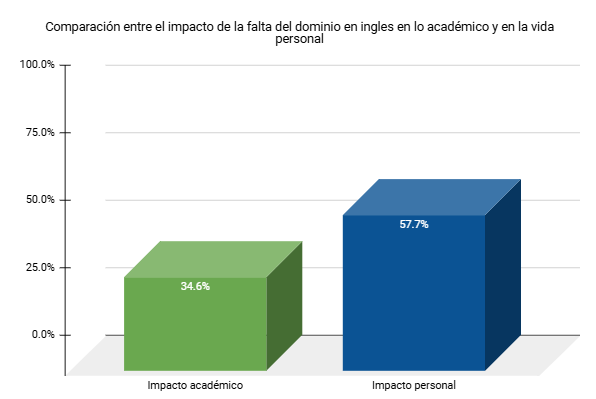
\includegraphics[width=0.8\linewidth]{Imagenes/Grafico impacto academico vs personal.png}
  \caption{Gráfico impacto académico vs personal}
  \label{fig:impactap}
\end{figure}

A partir de la \autoref{fig:impactap} podemos ver que el impacto de la falta de dominio del inglés es más significativo en la vida personal, con un 57.7\%, en comparación con el ámbito académico, que presenta un 34.6\%. Esto indica que las habilidades en inglés influyen mayoritariamente en situaciones personales y cotidianas que en el rendimiento académico. Sin embargo, no hay que ignorar el impacto académico, ya que también es significativo y afecta a una proporción considerable de la población.

\begin{figure}[H]
  \centering
  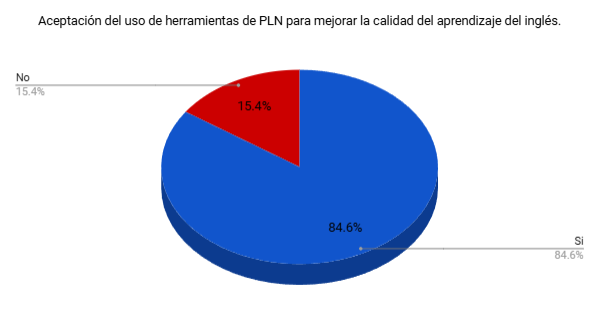
\includegraphics[width=0.8\linewidth]{Imagenes/Grafico 2 aceptacion del pln.png}
  \caption{Gráfico aceptación de herramientas de PLN}
  \label{fig:aceptpln}
\end{figure}


En la \autoref{fig:aceptpln} se puede evidenciar una alta aceptación del uso de herramientas de PLN para mejorar la calidad del aprendizaje del inglés, con un 84.6\% de personas a favor. Aunque una minoría del 15.4\% no está de acuerdo, la amplia mayoría sugiere un reconocimiento significativo del valor que estas herramientas pueden aportar en el proceso educativo.
\newpage
\begin{figure}[H]
  \centering
  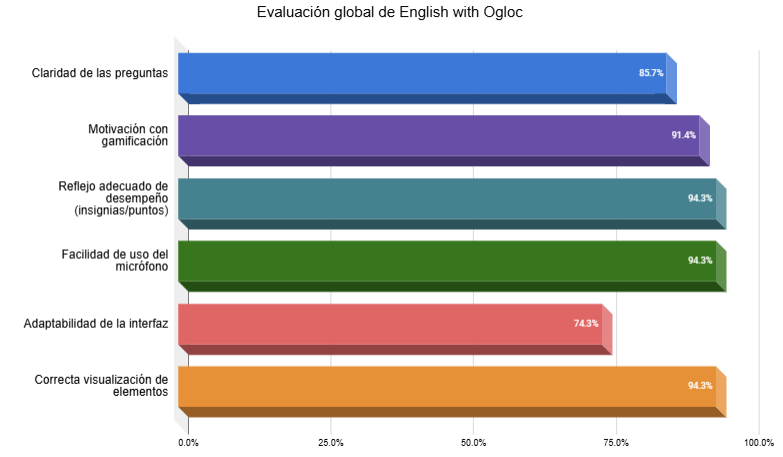
\includegraphics[width=0.9\linewidth]{Imagenes/Grafico 3 barras aceptacion general del prototipo.png}
  \caption{Gráfico evaluación global del prototipo}
  \label{fig:evalprot}
\end{figure}

En la \autoref{fig:evalprot} muestra una evaluación positiva del prototipo web en varias áreas clave, con alta satisfacción en el reflejo adecuado del desempeño y la correcta visualización de elementos (ambos con 94.3\%). La motivación con gamificación también es bien valorada, con un 91.4\%. Aunque la adaptabilidad de la interfaz tiene la valoración más baja con un 74.3\%, sigue siendo aprobada por la mayoría, indicando un desempeño sólido en general.
